\usepackage[english]{babel}
\usepackage[utf8]{inputenc}
\usepackage{lmodern}
\usepackage{amsmath,amssymb,amsfonts}
\usepackage{url}

% only presentation 
\mode<presentation>
{
  \usetheme{default}
  \setbeamercovered{transparent}
  \usefonttheme{structurebold}
  \setbeamertemplate{theorems}[numbered]
  \usepackage{amscd}
}

\usepackage{enumerate}
\usepackage{stmaryrd}
\usepackage{calc}
\usepackage{lmodern}
\usepackage{expl3,xparse}
\usepackage{lstlinebgrd} 

\ExplSyntaxOn
\NewDocumentCommand \lstcolorlines { O{green} m }
{
 \clist_if_in:nVT { #2 } { \the\value{lstnumber} }{ \color{#1} }
}
\ExplSyntaxOff

% Title definition
\title{DUNE PDELab Tutorial 06\\
{\small  Paralleles Rechnen}}
\author{Olaf Ippisch}
\institute[]
{
  Institut für Mathematik, TU Clausthal\\
  Erzstr. 1, D-38678 Clausthal-Zellerfeld \\[6pt]
}
\date[\today]{\today}


% logo nach oben
\mode<presentation>
{
% No navigation symbols and no lower logo
\setbeamertemplate{sidebar right}{}

% logo
\newsavebox{\logobox}
\sbox{\logobox}{%
    \hskip\paperwidth%
    \rlap{%
      % putting the logo should not change the vertical possition
      \vbox to 0pt{%
        \vskip-\paperheight%
        \vskip0.35cm%
        \llap{\insertlogo\hskip0.1cm}%
        % avoid overfull \vbox messages
        \vss%
      }%
    }%
}

\addtobeamertemplate{footline}{}{%
    \usebox{\logobox}%
}
}

%%%%%%%%%%%%%%%%%%%%%%%%%%%%%%%%%%%%%%%%%%%%%%%%%%%%%%%%%%%%%%%%%%%%%%%%%%%%%%%%
%%%%%%%%%%%%%%%%%%%%%%%%%%%%%%%%%%%%%%%%%%%%%%%%%%%%%%%%%%%%%%%%%%%%%%%%%%%%%%%%
%
% now comes the individual stuff lecture by lecture
%
%%%%%%%%%%%%%%%%%%%%%%%%%%%%%%%%%%%%%%%%%%%%%%%%%%%%%%%%%%%%%%%%%%%%%%%%%%%%%%%%
%%%%%%%%%%%%%%%%%%%%%%%%%%%%%%%%%%%%%%%%%%%%%%%%%%%%%%%%%%%%%%%%%%%%%%%%%%%%%%%%

\begin{document}

\begin{onlyenv}<article>
\maketitle
\end{onlyenv}

\frame{\titlepage}

%%%%%%%%%%%%%%%%%%%%%%%%%%%%%%%%%%%%%%%%%%%%%%%%%%%%%%%%%%%%%%%%%%%%%%%%%%%%%%%%
%%%%%%%%%%%%%%%%%%%%%%%%%%%%%%%%%%%%%%%%%%%%%%%%%%%%%%%%%%%%%%%%%%%%%%%%%%%%%%%%

\section{Introduction}

\subsection{Why Parallel Computing?}

\begin{frame}
\frametitle<presentation>{Why Parallel Computing?}

\begin{itemize}
\item The speed of individual computer cores is not increasing essentially since some years due to
\begin{itemize}
\item Power wall
\item Memory wall
\item Instruction level parallelism (ILP) wall 
\end{itemize}
\item However, the number of cores is increasing. Quad-cores are the rule, up to 260-core processors are available
\item Several multi-core processors can be used on one mainboard (e.g. two 10-core processors)
\item Computer cluster with several multi-core multi-processor servers are affordable even for small companies
\end{itemize}

\end{frame}


\begin{frame}
\frametitle<presentation>{Why Parallel Computing?}

The worlds three fastest computers have 
\begin{itemize}
\item Sunway TaihuLight, Wuxi, China: 93.0 PFlop/s\\
10'649'600 cores: 
\begin{itemize}
\item 40'960 SW26010 processors, 260 cores\\
\end{itemize}
\item Tianhe-2, Guangzhou, China: 33.8 PFlop/s\\
3'120'000 cores:
\begin{itemize}
\item 32'000 Intel Xeon 12-core processors
\item 48'000 Intel Phi 57-core accelerator cards
\end{itemize}
\item Titan, Oak Ridge National Laboratory, U.S.A.: 17.6 PFlop/s\\
299'008 cores:
\begin{itemize}
\item 18'688 AMD Opteron 16-core processors
\item 18'688 NVIDIA Kepler K20X GPU accelerator cards
\end{itemize}
\end{itemize}

\end{frame}
%-----------------------------------------------------------------------------

\subsection{Architectures of Parallel Computers}

\begin{frame}
\frametitle<presentation>{Architectures of Parallel Computers}
\begin{itemize}
\item Shared-memory computing: all cores have access to the whole memory
\begin{itemize}
\item Uniform memory access architecture (UMA): \\
 access to every memory location from every process takes the
same amount of time (some multi-core CPUs)
\item Non-uniform memory access architecture (NUMA): \\
memory is associated with a processor or a group of processor cores but address space is
global. Local memory can be accessed faster than memory attached
to other processes (some multi-core CPUs, multi-processor servers)
\end{itemize}
\item Message passing architecture (MP): \\
 each process can only access local memory, information is exchanged
between processes with messages send over a network (computer clusters, super computer)
\end{itemize}
\end{frame}


\begin{frame}
\frametitle{Comparison of Architectures by Example}
\begin{itemize}
\item Given vectors $\mathbf{x},\mathbf{y}\in\mathbb{R}^N$, compute scalar product $s =
  \sum_{i=0}^{N-1} \mathbf{x}_i \, \mathbf{y}_i$:
\begin{itemize}
\item[(1)] Subdivide index set into $P$ pieces.
\item[(2)] Compute $s_p=\sum_{i=pN/P}^{(p+1)N/P-1} \mathbf{x}_i \, \mathbf{y}_i$ in
  parallel.
\item[(3)] Compute $s = \sum_{i=0}^{P-1} s_i$.
\end{itemize}
\item \textit{Uniform memory access architecture}: Store vectors as in
  sequential program:
\begin{center}
  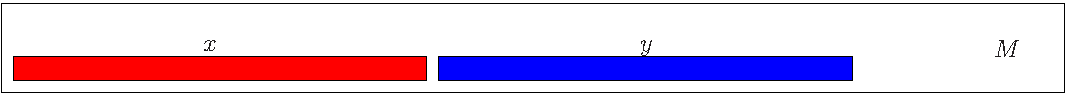
\includegraphics[width=0.9\textwidth]{umalayout}
\end{center}
\item \textit{Nonuniform memory access architecture}: Distribute
  data to the local memories:
\begin{center}
  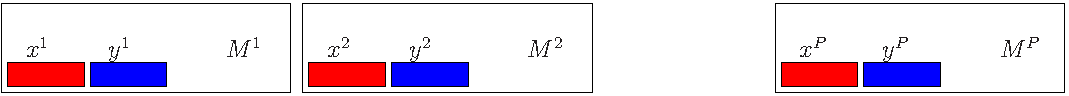
\includegraphics[width=0.9\textwidth]{numalayout}
\end{center}
\item \textit{Message passing architecture}: Same as for NUMA!
\item Parallelisation effort for NUMA and MP is almost the same.
\item Distributing data structures is hard and not automatic in
  general.
\end{itemize}
\end{frame}


\subsection{Message Passing}
\begin{frame}
\frametitle<presentation>{Message Passing}

\begin{itemize}
\item Users view: Copy (contiguous) memory block from one address space to the
  other.
\item During transmission the message is subdivided into individual packets.
\item Network is packet-switched.
\item A packet consists of an envelope and
  the data:
\begin{center}
  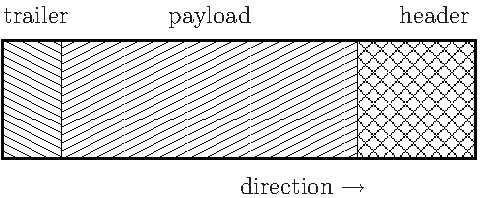
\includegraphics[width=0.49\textwidth]{paket}
\end{center}
\item Header: Destination, size and kind of data.
\item Payload: Size ranges from some bytes to kilobytes.
\item Trailer: e.g. checksum for error detection.
\end{itemize}
\end{frame}

%----------------------------------------------------------------------------------------
\begin{frame}
\frametitle{The Message Passing Interface (MPI)}

\begin{itemize}
\item Portable Library with functions for message exchange between processes
\item Developed 1993-94 by a international board
\item Available on nearly all computer platforms
\item Free Implementations also for Linux Clusters: {\bfseries MPICH}
 and {\bfseries OpenMPI} \footnote{\tiny \url{http://www-unix.mcs.anl.gov/mpi/mpich} and \url{http://www.open-mpi.org/}}
\item Properties of MPI:
\begin{itemize}
\item library with C- and Fortran bindings (no language extension)
\item large variety of point-to-point communication functions
\item global communication
\item data conversion for heterogeneous systems
\item subset formation and topologies possible
\end{itemize}
\end{itemize}
\end{frame}

\subsection{Strong Scalability Example}
\begin{frame}
\frametitle<presentation>{Strong Scalability of 3D Parallel Computation}
\begin{center}
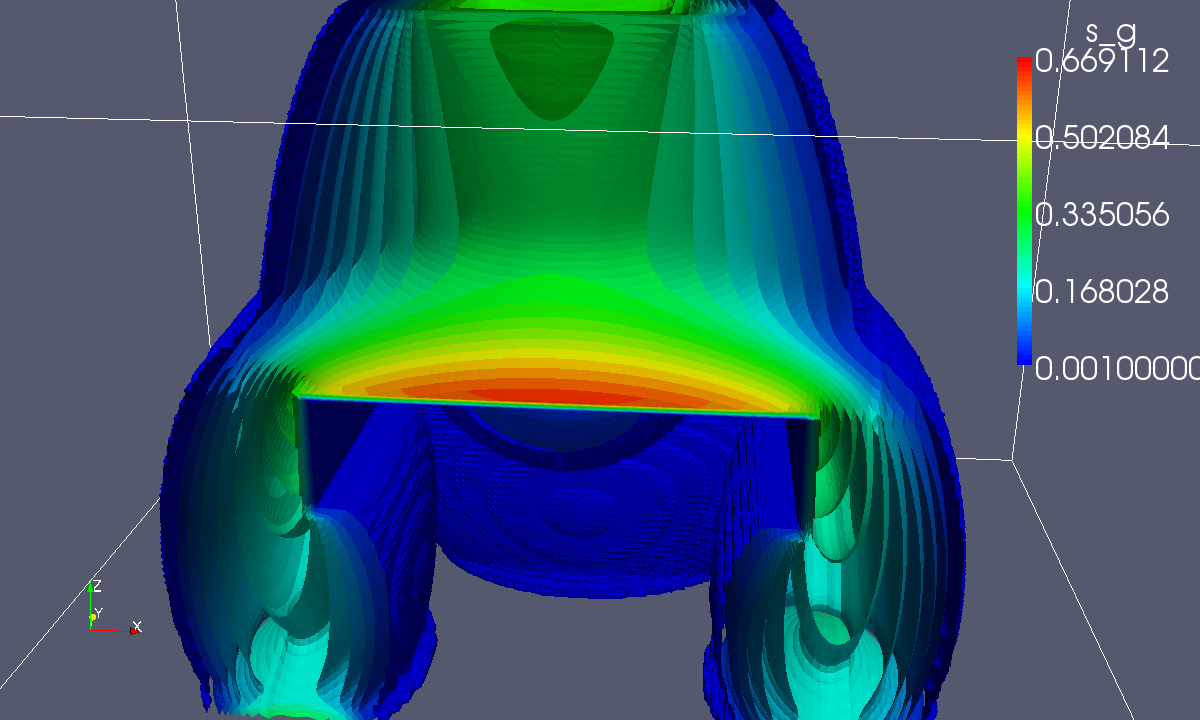
\includegraphics[width=0.9\textwidth]{dnapl-3d-het-iso}\\
3D DNAPL Infiltration
\end{center}
\end{frame}


\begin{frame}
\frametitle<presentation>{Strong Scalability of 3D Parallel Computation}
Simulation of a DNAPL infiltration with a coarse lense on a grid with  $160 \times 160 \times 96$
unknowns on a server with 4$\times$12  AMD Magny Cours, 2.1~GHz, 12$\times$0.5MB L2, 12MB
L3 processors.

Computation time for one time step with BiCGStab + AMG prec.:
\begin{center}
\begin{tabular}{r|rrr|rr|rr}
\hline
P  & \#IT(max) & $T_{it}$ & S & $T_{asm}$ & S & $T_{total}$ & S \\
\hline
 1  &  6.5 & 4.60 &      - &  43.7 &      - & 713.8 &    - \\
 4  &  10  & 1.85 &   2.5 &  17.5 &   2.5 & 295.9 & 2.4 \\
 8  &  9    & 0.63 &   7.3 &    8.4 &   5.2 & 127.1 & 5.6 \\
16 &  9.5 & 0.40 & 11.5 &    4.1 & 10.7 &   73.1 & 9.8 \\
32 &  15  & 0.27 & 17.0 &    1.9 & 23.0 &   43.5 & 16.4 \\
\hline
\end{tabular}
\end{center}

Comparison with T3E from 1999
\begin{center}
\begin{tabular}{r|rrrr}
\hline
Machine  & Cells & Time steps & Newton steps & $T_{total}$ \\
\hline
256 T3E        & 2621440 &  50 & 264 & 14719\\
16 Cores AMD & 2457600 & 50 & 231 & 2500\\
\hline
\end{tabular}
\end{center}
\vfill
\end{frame}


\section{Domain Decomposition}
\begin{frame}
  \frametitle<presentation>{Domain Decomposition}

  \begin{itemize}
  \item partition a problem by splitting the domain into smaller subdomains
  \item each part is solved by a different process
  \item goes back to an idea of H.A. Schwarz who in 1890 presented a method to prove the existence of
        solutions of the Laplace equation on ``complicated'' domains.
  \item Different variants:
    \begin{itemize}
    \item overlapping domain decomposition
    \item non-overlapping domain decomposition
    \end{itemize}
  \end{itemize}

  \begin{center}
    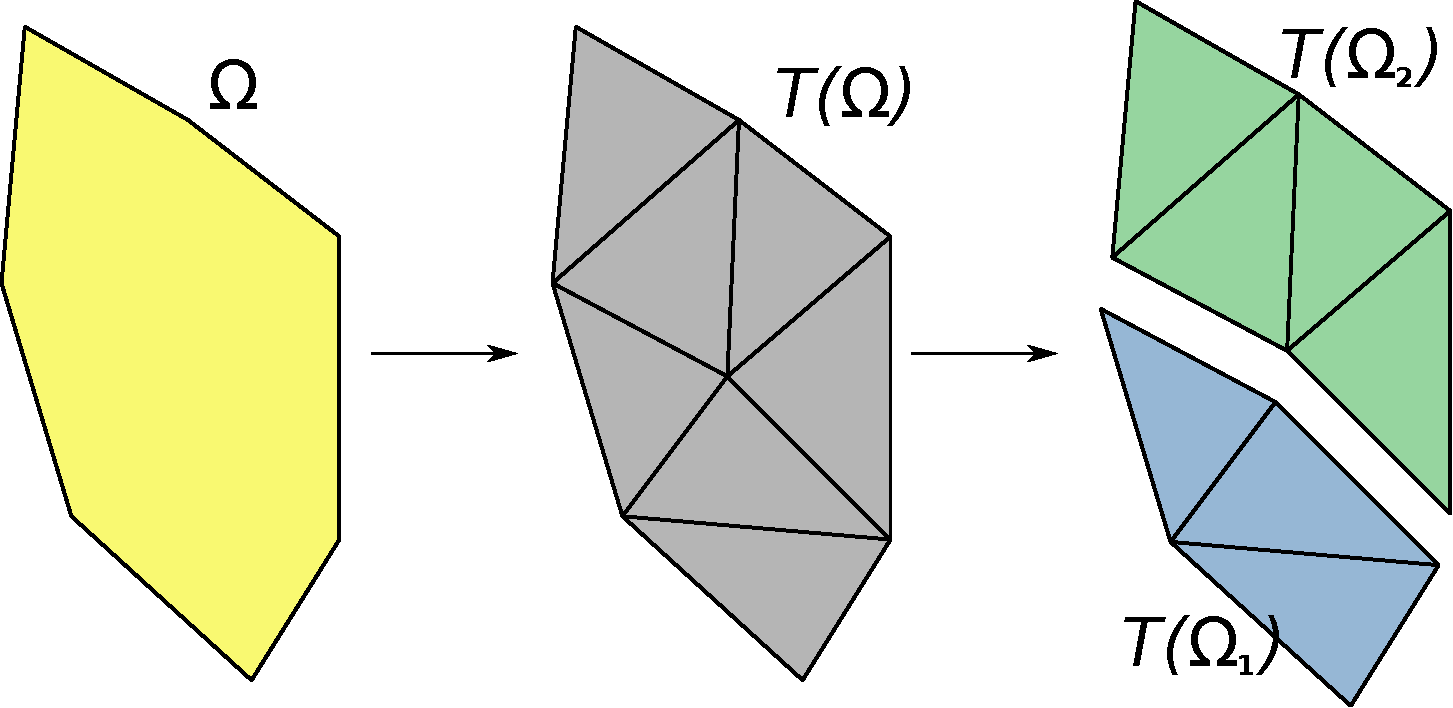
\includegraphics[width=.6\linewidth]{dd}
  \end{center}

\end{frame}

\subsection{Nonoverlapping Domain Decomposition}
\begin{frame}
  \frametitle<presentation>{Nonoverlapping Domain Decomposition}

  \begin{columns}
    \begin{column}{0.6\linewidth}
      % In overlapping domain decomposition methods, the subdomains
      % overlap by more than the interface. Overlapping domain
      % decomposition methods
      % include the Schwarz alternating method and the additive
      % Schwarz
      % method. Many domain decomposition methods can be written and
      % analyzed as a special case of the abstract additive Schwarz
      % method.

      \begin{itemize}
      \item Given a domain $\Omega\subseteq\mathbb{R}^d$
        % and a triangulation $T(\Omega) = \{E\}$
        % \item partition the cells $E$ such that there is exactly one
        %   process with $E \in T(\Omega_i)$
      \item partition $\Omega$ into \emph{non-overlapping}
        sub-domains:
        \[
        \Omega_i\colon\quad \bigcup_{i=1}^p \overline{\Omega}_i = \overline{\Omega}, \quad
        \Omega_i\cap\Omega_j=\emptyset \;\forall i\ne j.
        \]
      \end{itemize}
    \end{column}
    \begin{column}{0.4\linewidth}
      \begin{onlyenv}<presentation>
        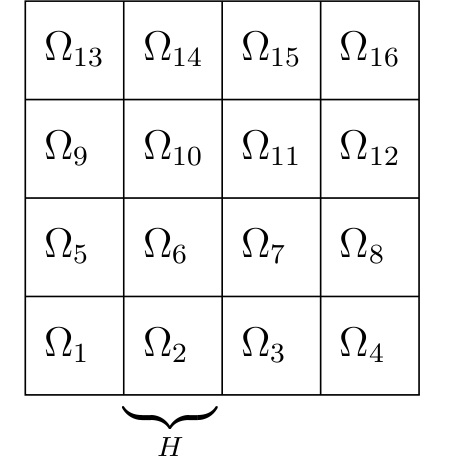
\includegraphics[width=0.6\linewidth]{konstr_n_uberl_str}
        \vskip5mm
        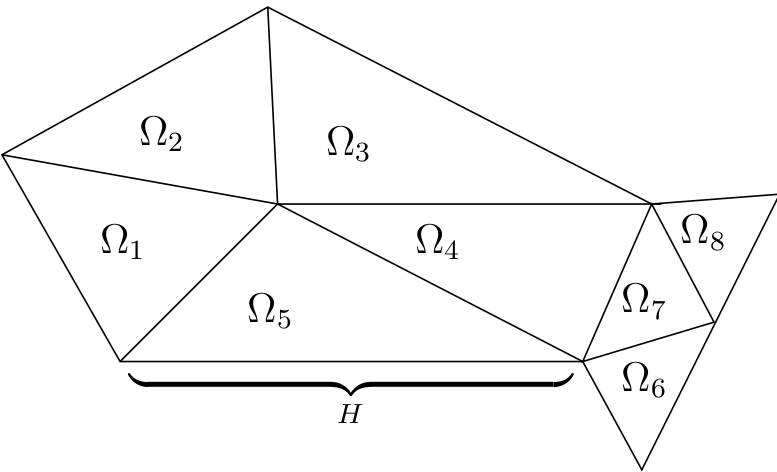
\includegraphics[width=0.9\linewidth]{konstr_n_uberl_unstr}
      \end{onlyenv}
      \begin{onlyenv}<article>
        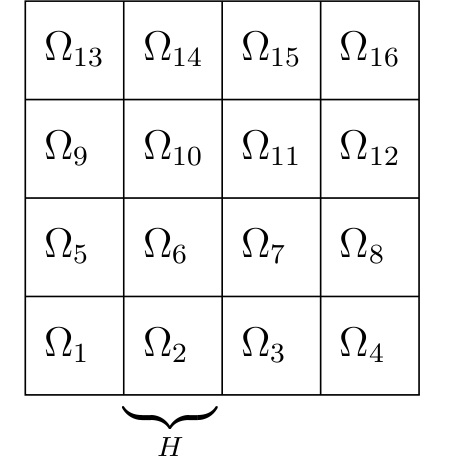
\includegraphics[width=0.25\linewidth]{konstr_n_uberl_str}
        \vskip5mm
        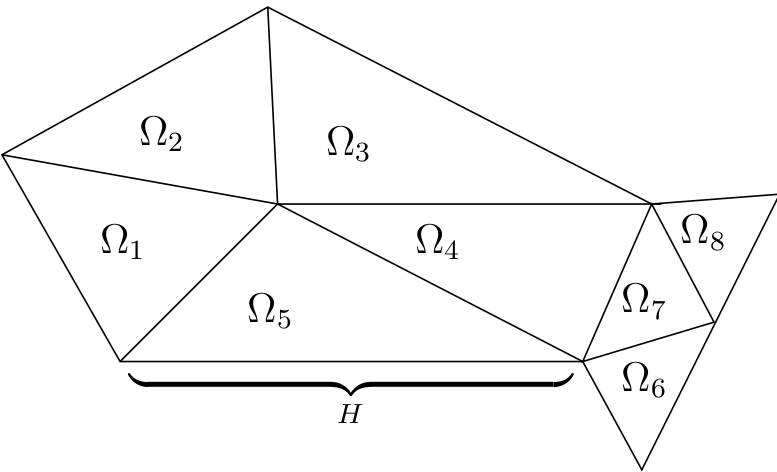
\includegraphics[width=0.36\linewidth]{konstr_n_uberl_unstr}
      \end{onlyenv}
    \end{column}
  \end{columns}
\end{frame}

\subsection{Overlapping Domain Decomposition}
\begin{frame}
  \frametitle<presentation>{Overlapping Domain Decomposition}

  \begin{columns}
    \begin{column}{0.6\linewidth}
      % In overlapping domain decomposition methods, the subdomains
      % overlap by more than the interface. Overlapping domain
      % decomposition methods
      % include the Schwarz alternating method and the additive
      % Schwarz
      % method. Many domain decomposition methods can be written and
      % analyzed as a special case of the abstract additive Schwarz
      % method.

      \begin{itemize}
      \item Extend each $\Omega_i$ by an overlap $\hat \Omega_i$ of width
        $\beta\cdot H$:
        \[
        \hat \Omega_i = \left\{ x\in\Omega \mid \mathsf{dist}(x,\Omega_i) < \beta\cdot H \right\}
        \]
      \end{itemize}
    \end{column}
    \begin{column}{0.4\linewidth}
      \begin{onlyenv}<presentation>
        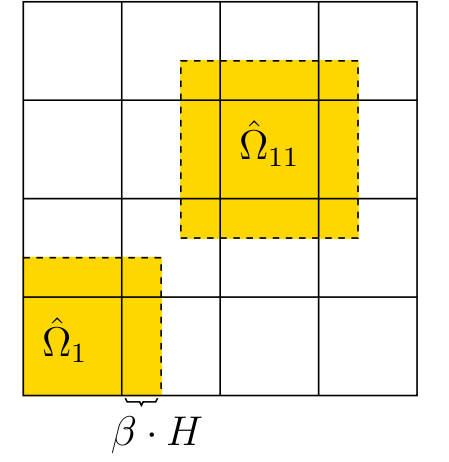
\includegraphics[width=0.6\linewidth]{konstr_uberl_str}
        \vskip5mm
        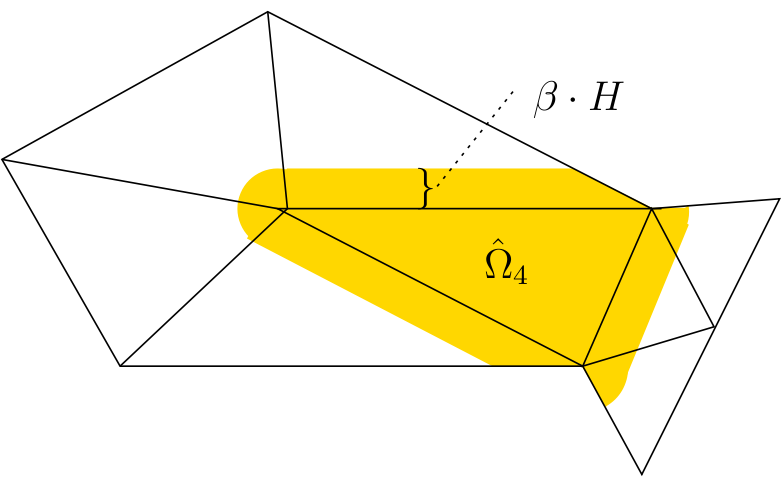
\includegraphics[width=0.9\linewidth]{konstr_uberl_unstr}
      \end{onlyenv}
      \begin{onlyenv}<article>
        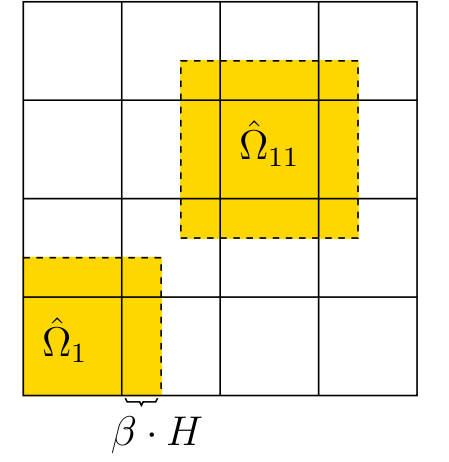
\includegraphics[width=.25\linewidth]{konstr_uberl_str}
        \vskip5mm
        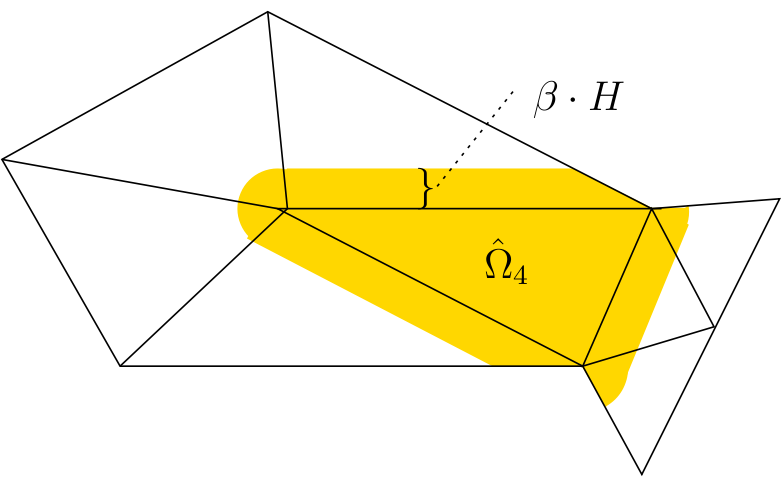
\includegraphics[width=.36\linewidth]{konstr_uberl_unstr}
      \end{onlyenv}
    \end{column}
  \end{columns}
\end{frame}

\section{Parallel Grids}

%-----------------------------------------------------------------------------

\begin{frame} \frametitle{Recapitulation: The Grid: A Container of Entities}

  In the DUNE sense a \emph{Grid} is a container of entities:

  \only<presentation>{\vspace*{5mm}}
  \begin{columns}
    \begin{column}{5mm}
    \end{column}
    \begin{column}{0.5\linewidth-5mm}
      \begin{onlyenv}<presentation>
        \includegraphics<1-2>[width=\linewidth]{entities}
        \includegraphics<3->[width=\linewidth]{entities_cd}
      \end{onlyenv}
      \begin{onlyenv}<article>
        \vspace*{2ex}
        ~\hfill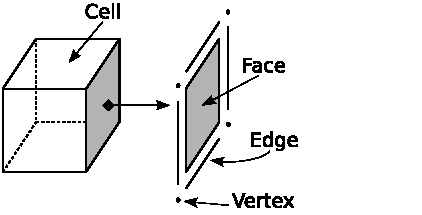
\includegraphics[width=0.4\linewidth]{entities}\hfill
        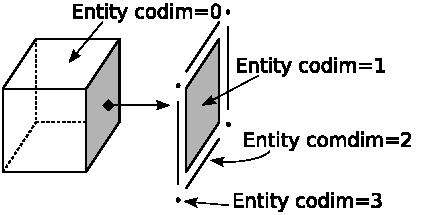
\includegraphics[width=0.4\linewidth]{entities_cd}\hfill~
      \end{onlyenv}
    \end{column}\hfill
    \begin{column}{0.5\linewidth}
      \begin{itemize}
      \item vertices \only<3->{\emph{(Entity codim = $d$)}},
      \item edges \only<3->{\emph{(Entity codim = $d-1$)}},
      \item faces \only<3->{\emph{(Entity codim = $1$)}},
      \item cells \only<3->{\emph{(Entity codim = $0$)}}, \ldots{}
      \end{itemize}
    \end{column}
  \end{columns}
  \only<presentation>{\vspace*{5mm}}

  \pause{In order to do dimension independent programming, we need a
    dimension independent naming for different entities.}
  \only<presentation>{\par}
  \pause{We distinguish entities according to their codimension.}
  \only<presentation>{\par}
  Entities of codim = $c$ contain subentities of codim = $c+1$. This
  gives a recursive construction down to codim = $d$.

\end{frame}

\begin{frame}
  \frametitle{Recapitulation: Iterators}
  Access to the entities of a grid is given by iterators provided by a \lstinline!GridView!. DUNE provides
  appropriate iterators for both \lstinline!LeafGridView! and \lstinline!LevelGridView!.
  \begin{columns}
    \begin{column}{0.47\linewidth}
      \begin{center}
        \begin{onlyenv}<article>
          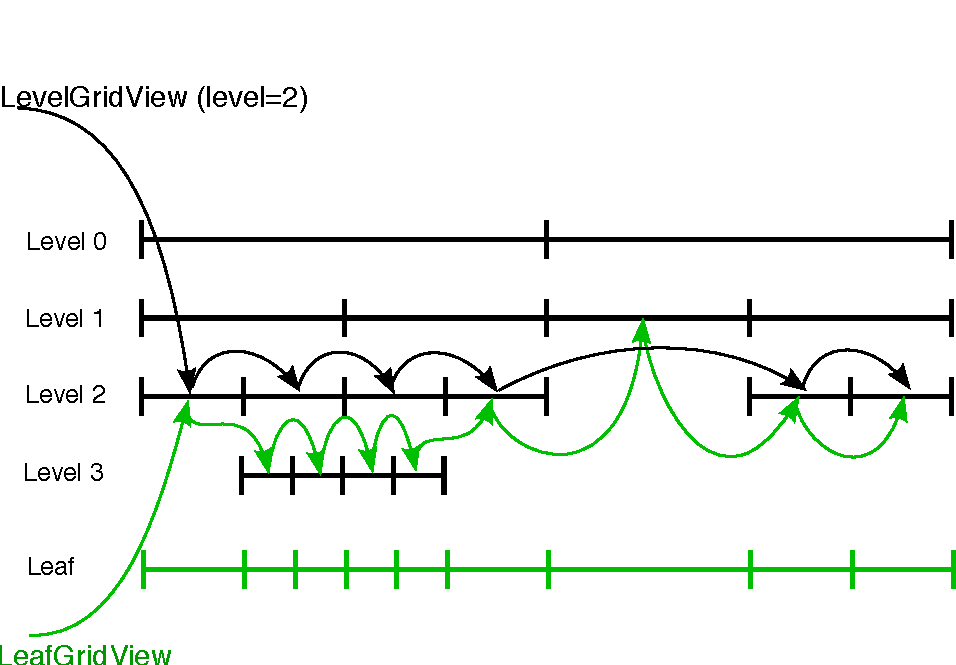
\includegraphics[width=0.7\linewidth]{iterators}
        \end{onlyenv}
      \end{center}
      \begin{onlyenv}<presentation>
        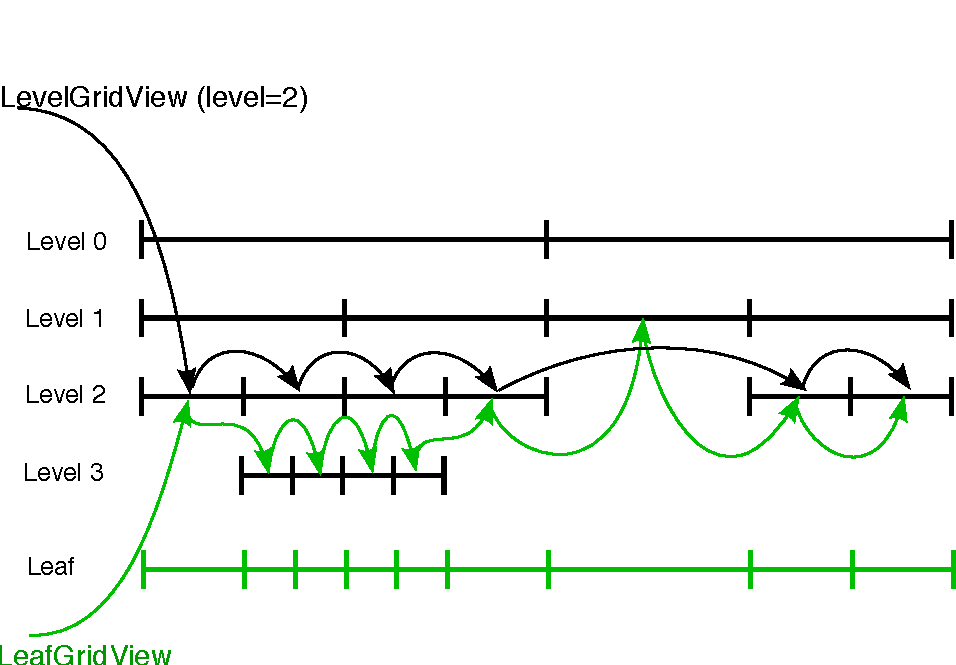
\includegraphics[width=\linewidth]{iterators}
      \end{onlyenv}
    \end{column}
    \begin{column}{0.53\linewidth}
      \lstinline!GridView::Codim<c>::Iterator!\\ iterates over codimension
        $c$ entities on a given view.
    \end{column}
  \end{columns}
\end{frame}

\begin{frame} \frametitle{Recapitulation: Entities}

  \structure{Iterating over a grid view, we get access to the entities.}

%  \begin{block}{}%
    \only<presentation>{\lstset{basicstyle=\scriptsize\ttfamily}}
      \lstinputlisting[breaklines=true]{entity.cc}%
%  \end{block}

%  \pause
  \begin{itemize}
  \item Entities cannot be modified.
  \item Entities can be copied and stored (but copies may be expensive).
%    \pause
  \item Entities provide topological and geometrical information.
  \end{itemize}
\end{frame}

\begin{frame}
  \frametitle<presentation>{Recapitulation: Entities}

  \structure{An Entity $E$ provides both topological information}
  \begin{itemize}
  \item Type of the entity (triangle, quadrilateral, etc.).
  \item Relations to other entities.
  \end{itemize}
  \structure{and geometrical information}
  \begin{itemize}
  \item Position of the entity in the grid.
  \end{itemize}

  \only<presentation>{\vfill}
%  \pause
  \begin{columns}
    \begin{column}{5mm}
    \end{column}
    \begin{column}{0.4\textwidth}
      \begin{center}
        \visible<presentation|1->{
          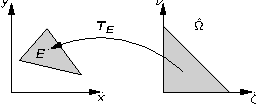
\includegraphics[width=\linewidth]{refelem-mapping}}\\
        \begin{onlyenv}<article>
          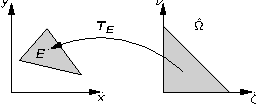
\includegraphics[width=0.6\linewidth]{refelem-mapping}\\
        \end{onlyenv}
        \centerline{\tiny Mapping from $\hat{\Omega}$ into global coordinates.}
      \end{center}
    \end{column}
    \begin{column}{0.5\textwidth}
      \structure{Entity $E$ is defined by\dots{}}
        \begin{itemize}
        \item Reference Element $\hat{\Omega}$
        \item Transformation $T_E$
        \end{itemize}
    \end{column}
  \end{columns}

  \only<presentation>{\vfill}
%  \pause
  \lstinline!GridView::Codim<c>::Entity!
  implements the entity concept.

\end{frame}

\subsection{Partition Types}
\begin{frame}[fragile]
\frametitle<presentation>{Partition Types}

\begin{itemize}
\item Each grid entity can be present on one or more processes.
\item Each entity on one process has a partition type, which can be determined
by the method\\
        \hspace*{1cm}\lstinline!entity.partitionType()!
\item The possible partition types are:\\
\end{itemize}
\begin{tabular}{ll}
  \em \bfseries interior
  & Entity is owned by the process\\
  \em \bfseries overlap & Entity is owned by a different process, but a full copy exists\\
  \em \bfseries ghost
  & Entity is owned by a different process, but a partial copy\\
  & exists\\
  \em \bfseries border
  & Boundary of interior. (only exists for entities with \\
  & codimension$>$0)\\
  \em \bfseries front
  & Boundary of interior+overlap if not {\em \bfseries border} (only exists for\\
  & entities with codimension$>$0)
\end{tabular}
\end{frame}


\begin{frame}[fragile]
\frametitle{Partition Types Example}
\begin{columns}[c]
\begin{column}{0.75\textwidth}

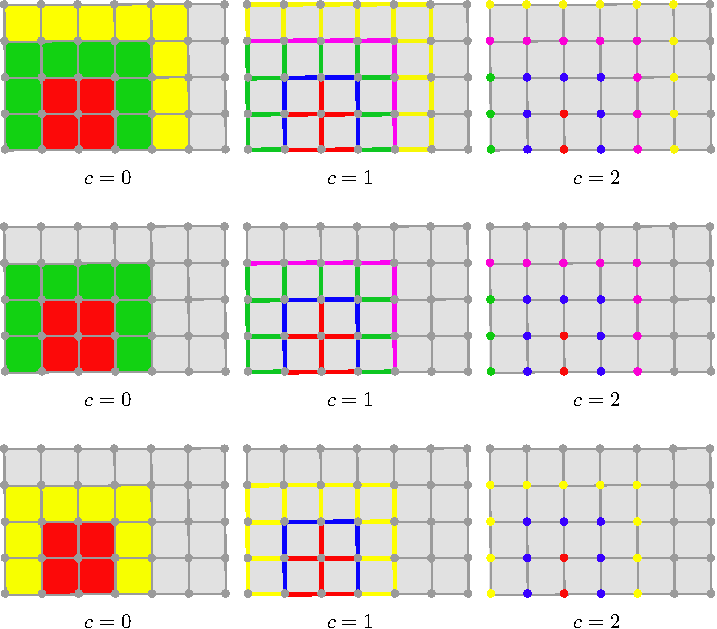
\includegraphics[width=\textwidth]{partitionsingle}
\end{column}
\begin{column}{0.25\textwidth}
\vskip0.5cm
\textbf{First row}: with overlap and ghosts\\
\textbf{Second row}: with overlap only\\
\textbf{Third row}: with ghosts only
\vskip5mm
\begin{center}
\begin{tabular}{|c|}
\hline\color{red} interior\\\hline
\color{green} overlap\\\hline
\color{yellow} ghost\\\hline
\color{blue} border\\\hline
\color{magenta} front\\\hline
\color{gray} not stored\\\hline
\end{tabular}
\end{center}
\end{column}
\end{columns}

\end{frame}

\subsection{Parallel Grids in Dune}

\begin{frame}
  \frametitle<presentation>{Parallel Grids in Dune}
  \begin{itemize}
  \item<1-> \lstinline!YaspGrid!
      \begin{itemize}
      \item structured
      \item 2D/3D
      \item arbitrary overlap
      \end{itemize}
  \item<2-> \lstinline!UGGrid!
      \begin{itemize}
      \item unstructured
      \item 2D/3D
      \item multi-element (e.g. tetrahedrons, pyramids, prisms and hexahedrons simultaneously in 3D)
      \item non-conforming/conforming refinement
      \item ghost cells
      \end{itemize}
  \item<3-> \lstinline!ALUGrid!
      \begin{itemize}
      \item unstructured
      \item 2D/3D
      \item either tetrahedral or hexahedral elements
      \item non-conforming refinement, conforming bisection refinement for 3D tetrahedral grid
      \item ghost cells (non-conforming grids only)
      \item full load-balancing
      \end{itemize}
  \end{itemize}
\end{frame}

\subsection{Iterators on a Parallel Grid}

\begin{frame}[fragile]
  \frametitle<presentation>{Iterators in a parallel Grid}
  \small
  Dune offers Iterators which only iterate over elements with certain partition types. The partition type can be specified as additional parameter in the range based for loop, e.g.
\begin{lstlisting}[breaklines=true,basicstyle=\ttfamily\small]
    for (const auto &cell : elements(gv,Dune::Partitions::Interior) {
    ...
    }
\end{lstlisting}

\lstinline!Dune::Partitions! contains the following partitions:\smallskip\\

    \begin{tabular}{ll}
      \lstinline!Interior! & interior entities only\\
      \lstinline!Border! & border entities only\\
      \lstinline!Overlap! & overlap entities only\\
      \lstinline!Front! & front entities only\\
      \lstinline!InteriorBorder! & interior entities plus border (identical to \\
     & \lstinline!Interior! for entities of  codimension==0)\\
      \lstinline!InteriorBorderOverlap! & interior, border and overlap entities\\
      \lstinline!InteriorBorderOverlapFront! & interior, border, overlap and front entities \\
      \lstinline!Ghost! & ghost entities only\\
      \lstinline!All! & all entities available to the process
    \end{tabular}
\end{frame}

\begin{frame}
  \frametitle{Example}
    \only<presentation>{\lstset{basicstyle=\scriptsize\ttfamily}}
  \lstinputlisting[breaklines=true]{iterators.cc}
\end{frame}

\begin{frame} \frametitle{Repetition: Intersections}

  \begin{columns}
    \begin{column}{0.4\linewidth}
      \begin{center}
        \includegraphics<presentation>[width=\linewidth]{intersection}
        \includegraphics<article>[width=0.45\linewidth]{intersection}
      \end{center}
    \end{column}
    \begin{column}{0.6\linewidth}
      \begin{itemize}
      \item Grids may be non conforming.
      \item Entities can intersect with neighbours and boundary.
      \item IntersectionIterators give access to intersections of
        an Entity in a given view.
      \item Intersections hold topological and
        geometrical information.
      \item Intersections depend on the view:
      \item \textbf{Note:} Intersections are always of
        codimension 1!
      \end{itemize}
    \end{column}
  \end{columns}

\end{frame}

\begin{frame} \frametitle{Intersection Interface}
  Iterating over intersections in entity $E$ yields an \lstinline!Intersection! to $E'$ with the methods:\bigskip

  \begin{columns}
    \begin{column}{0.4\linewidth}
      \begin{center}
        \includegraphics<presentation>[width=\linewidth]{intersection}
      \end{center}
    \end{column}
    \begin{column}{0.6\linewidth}
    \only<presentation>{\scriptsize}
    \begin{tabular}{l|p{0.3\linewidth}}
      \hline
      Method name & Result \\\hline
      \lstinline!boundary! &
      Boolean \\
      \lstinline!neighbor! &
      Boolean \\
      \lstinline!inside! &
      Entity $E$ \\
      \lstinline!outside! &
      Entity $E'$ \\
      \lstinline!geometry! &
      Geometry $T_{I}$ \\
      \lstinline!geometryInInside! &
      Geometry $T_{I,E}$ \\
      \lstinline!geometryInOutside! &
      Geometry $T_{I,E'}$ \\
      \lstinline!unitOuterNormal! &
      outer normal $n$, $|n| = 1$\\
      \lstinline!centerUnitOuterNormal! &
      outer normal at \mbox{geometry().center()}
      \\\hline
    \end{tabular}
    \end{column}
  \end{columns}

\end{frame}

%-----------------------------------------------------------------------------
\begin{frame}
\frametitle{Intersections and Domain Decomposition}
\begin{itemize}
\item On each intersection there exists a method \lstinline!neighbor()!. This method returns \lstinline!true! if there is a
neighbor available on the same process (even if it is a ghost).
\item The method \lstinline!boundary()! only returns \lstinline!true! at the domain boundary (even if the grid is periodic at this boundary) not at a process boundary.
\item If there is no neighbor but also no domain boundary, there is a process boundary.
\end{itemize}
\end{frame}

\begin{frame} \frametitle{Example}
\only<presentation>{\lstset{basicstyle=\scriptsize\ttfamily}}
  \lstinputlisting[breaklines=true]{intersection.cc}
\end{frame}

\subsection{Grid-Distribution and Load-Balancing}
\begin{frame}[fragile]
  \frametitle<presentation>{Load-Balancing}
  \begin{itemize}
  \item parallelization only scales well if all processes have the
    same work load\\
    $\Rightarrow$ well balanced grids necessary
  \item adaptation leads to unbalanced work load
  \item only 3D ALUGrid provides a fully working method to re-balance the work load after grid adaptation
  \begin{description}[123]
  \item[\ttfamily loadBalance(DataHandle \&data)]:\\
    re-balances a parallel grid, optionally sends also user data
  \item[\ttfamily DataHandle]:\\
    works like the data handle for the communicate methods
  \end{description}
   \item with UGGrid you can initialize a coarse grid and then call \lstinline!loadBalance! before starting the
         computation.
  \end{itemize}
\end{frame}

\begin{frame}[fragile]
  \frametitle{Grid-Distribution with YaspGrid}
With YaspGrid you can determine how the grid is partitioned (adaptive grid refinement and load-balancing are not possible as it is a structured grid) by writing a class derived from
\lstinline!Dune::YLoadBalance<dim>!

\only<presentation>{\lstset{basicstyle=\scriptsize\ttfamily}}
\begin{lstlisting}[breaklines=true]
template<int dim>
class YaspPartition : public Dune::YLoadBalance<dim>
{
  public:
    typedef Dune::FieldVector<int, dim>  iTupel;
    void loadbalance (const iTupel& size, int P, iTupel& dims) const
    {
      dims[0] = 1;
      dims[1] = P;
    }
};
\end{lstlisting}
\only<presentation>{\lstset{basicstyle=\normalsize\ttfamily}}
\end{frame}

\begin{frame}[fragile]
  \frametitle<presentation>{Grid-Distribution with YaspGrid}
Now you can pass the object to the constructor during grid creation
\begin{lstlisting}[breaklines=true]
Dune::FieldVector<int,2> n(10);
Dune::FieldVector<double,2> upper(1.0);
Dune::FieldVector<bool,2> periodic(false);
int overlap = 1;
YaspPartition<2> yp;
YaspGrid<2> grid(upper,n,periodic,overlap,&yp);
\end{lstlisting}
\end{frame}

\section{Communicating Data with Dune}
\begin{frame}[fragile]
  \frametitle<presentation>{Communicating Data with Dune}

%% local index

  \begin{itemize}
  \item Data is associated with grid entities using an \texttt{IndexSet}.
  \item The index set provides indices for all entities stored by the process (i.e. the \lstinline!Dune::Partitions::All!)
  \item Data is stored locally.
  \item Algorithms may require data exchange e.g. for synchronization or the calculation of updates
  \item Dune provides methods for the communication of data and methods for collective communication
  \end{itemize}

\end{frame}


\subsection{DUNE Lowlevel Communication API}
\begin{frame}[fragile]
  \frametitle<presentation>{DUNE Lowlevel Communication API}

  \texttt{GridView} provides a method for the communication between processes
\only<presentation>{\lstset{basicstyle=\scriptsize\ttfamily}}
    \begin{lstlisting}
template<class DHImp, class DataType>
void communicate (CommDataHandleIF<DHImp, DataType> &datahandle,
                  InterfaceType interface,
                  CommunicationDirection dir) const;
    \end{lstlisting}
\only<presentation>{\lstset{basicstyle=\normalsize\ttfamily}}
where
    \begin{itemize}
    \item \lstinline!CommDataHandleIF!\\
      is a user defined class describing what data should be communicated. The class has to provide methods to assemble the data on the
      source process and write distribute the data on the target process (see exercises).
    \end{itemize}
\end{frame}


\begin{frame}[fragile]
  \frametitle<presentation>{DUNE Lowlevel Communication API}
  \begin{onlyenv}<presentation>
\only<presentation>{\lstset{basicstyle=\scriptsize\ttfamily}}
    \begin{lstlisting}
template<class DHImp, class DataType>
void communicate ( CommDataHandleIF<DHImp, DataType> &datahandle,
                   InterfaceType interface,
                   CommunicationDirection dir ) const;
    \end{lstlisting}
\lstset{basicstyle=\normalsize\ttfamily}
where
    \end{onlyenv}
    \begin{itemize}
    \item \lstinline!InterfaceType!\\
    Determines the partition type of the entities to be sent and received. With \lstinline!InteriorBorder_InteriorBorder_Interface! only
border entities are sent. With \lstinline!All_All_Interface!,
    \lstinline!InteriorBorder_All_Interface! and
    \lstinline!Overlap_All_Interface! all entities, only interior and border entities or only overlap entities are sent. Only processes with common
data communicate and only the entities present on both processes are included in the communication.
    \item \lstinline!CommunicationDirection!
      The direction of the communication can be changed with either \lstinline!ForwardDirection! or
      \lstinline!BackwardDirection!
    \end{itemize}
\end{frame}



\subsection{Collective Communication}

\begin{frame}[fragile]
  \frametitle<presentation>{Collective Communication}
  \begin{itemize}
  \item parallel computations require global communication (e.g. sum(defect) or $\min(\Delta t)$
        and synchronization (e.g. a barrier needed for a timing)
  \item You can get a collective communicator object by the following method of a \lstinline!GridView!:
    \lstinline!  const CollectiveCommunication & comm () const;!
  \end{itemize}
\vfill
\vfill
\vfill
\vfill
\vfill
\vfill

\end{frame}

\begin{frame}[fragile]
  \frametitle<presentation>{Collective Communication}
The class  \lstinline!Dune::Grid::CollectiveCommunication! provides comfortable access to a lot of MPI methods, e.g.\medskip

    \begin{tabular}{l|p{7cm}}
      \hline
      Method name & Description\\\hline
      \lstinline!rank! & obtain number (rank) of this process\\
      \lstinline!size! & obtain number of processes \\
      \lstinline!barrier! & wait until all process arrived at the barrier\\
      \lstinline!min! & global min of local values\\
      \lstinline!max! & global max of local values\\
      \lstinline!sum! & global sum of local values\\
      \lstinline!allreduce! & Compute something over all processes for each component of an array \\
      &and return result in every process\\
      \lstinline!broadcast! & broadcast from one process to all other processes\\
      \lstinline!scatter! & scatter individual data from root process to all other tasks\\
      \lstinline!gather, allgather! & gather data on root process (and distribute it to all other tasks)\\
      \hline
    \end{tabular}

\end{frame}

\begin{frame}
  \frametitle{Example}
\only<presentation>{\lstset{basicstyle=\small\ttfamily}}
\lstinputlisting[lastline=12]{communicate.cc}
\end{frame}

\subsection{MPIHelper}
\begin{frame}[fragile]
  \frametitle<presentation>{MPIHelper}
  Dune parallel programs use a tool to help in setting up and handling the
parallel communication with MPI. It also takes care that the parallel program
is finished in a defined way. It is called \lstinline!MPIHelper!. It has to be
created at the very beginning of the program
using the \lstinline!instance! method of the \lstinline!Dune::MPIHelper! class.
\only<presentation>{\lstset{basicstyle=\scriptsize\ttfamily,breaklines=true}}
\lstinputlisting[lastline=12,breaklines=true]{example01_main.hh}

\end{frame}

\begin{frame}[fragile]
  \frametitle<presentation>{MPIHelper}
  \begin{itemize}
  \item MPIHelper provides the methods\medskip

    \only<presentation>{\scriptsize}
\only<presentation>{\lstset{basicstyle=\scriptsize\ttfamily}}    \begin{tabular}{l|l}
      \hline
      Method name & Description\\\hline
      \lstinline!rank! & obtain number (rank) of this process\\
      \lstinline!size! & obtain number of processes \\
      \hline
    \end{tabular}\medskip
    \only<presentation>{\normalsize}
  \item MPIHelper provides the static methods\medskip
  
    \only<presentation>{\scriptsize}
\only<presentation>{\lstset{basicstyle=\scriptsize\ttfamily}}    \begin{tabular}{l|p{6cm}}
      \hline
      Method name & Description\\\hline
      \lstinline!getCommunicator! & get communicator to exchange data
      with\\ & all process (\lstinline!MPI_COMM_WORLD!)\\
      \lstinline!getLocalCommunicator! & get communicator to exchange data with\\& the local process only (\lstinline!MPI_COMM_SELF!)\\
      \lstinline!getCollectiveCommunication! & get collective communication object for \lstinline!MPI_COMM_WORLD!\\
      \lstinline!instance! & get access to the helper singleton\\
      \hline
    \end{tabular} \medskip
    \only<presentation>{\normalsize}
   \item MPIHelper additionally provides an \lstinline!enum! \lstinline!isFake! which is \lstinline!true! if the program was compiled
without MPI support
 \end{itemize}
\end{frame}

\subsection{Norms and Scalar-Products on Parallel Grids}

\begin{frame}[fragile]
  \frametitle<presentation>{Norms and Scalar-Products on Parallel Grids}
If you have a parallel grid and for some reason want to calculate norms or scalar products of vectors associated with degrees of freedom, you cannot calculate them directly, as border entities exist on more than one process. 

For an overlapping grid you need the class \lstinline!OverlappingScalarProduct!. Additionally you need the auxiliary class \lstinline!ISTL::ParallelHelper!. 
\only<presentation>{\lstset{basicstyle=\scriptsize\ttfamily}}
\begin{lstlisting}[breaklines=true]
std::vector<double> dataVector(gv.indexSet().size(dim));
// obtain data from some calculations
Dune::PDELab::ISTL::ParallelHelper<GFS> parHelper(gfs);
Dune::PDELab::OverlappingScalarProduct<GFS,std::vector<double>> ovlpScalProd(gfs,parHelper);
// calculate norm
norm=ovlpScalProd.norm(dataVector);
\end{lstlisting}
\end{frame}

\begin{frame}[fragile]
  \frametitle<presentation>{Norms and Scalar-Products on Parallel Grids}
For a non-overlapping grid the respective class is 
\lstinline!NonoverlappingScalarProduct!:
\only<presentation>{\lstset{basicstyle=\scriptsize\ttfamily}}
\begin{lstlisting}[breaklines=true]
std::vector<double> dataVector(gv.indexSet().size(dim));
// obtain data from some calculations
Dune::PDELab::ISTL::ParallelHelper<GFS> parHelper(gfs);
Dune::PDELab::NonoverlappingScalarProduct<GFS,std::vector<double>> novlpScalProd(gfs,parHelper);
// calculate norm via scalar product
double norm=sqrt(novlpScalProd.dot(dataVector,dataVector));
\end{lstlisting}
\end{frame}


\section{Parallel PDELab}

\begin{frame}
  \frametitle<presentation>{Parallel PDELab}
Parallel computing in PDELab is very easy.
  \begin{itemize}
  \item Go parallel by choosing
    \begin{enumerate}
    \item a suitable parallel grid,
    \item the correct constraints for the discretization of
      the PDE (either\newline \lstinline!OverlappingConformingDirichletConstraints! or\newline \lstinline!NonoverlappingConformingDirichletConstraints<GV>!) , and
    \item a suitable and matching parallel solver backend of the
      PDELab backend.
    \end{enumerate}
  \end{itemize}
\end{frame}

\subsection{Parallel Solver Backends}
\begin{frame}
  \frametitle<presentation>{Building Blocks for Parallel Solvers}
  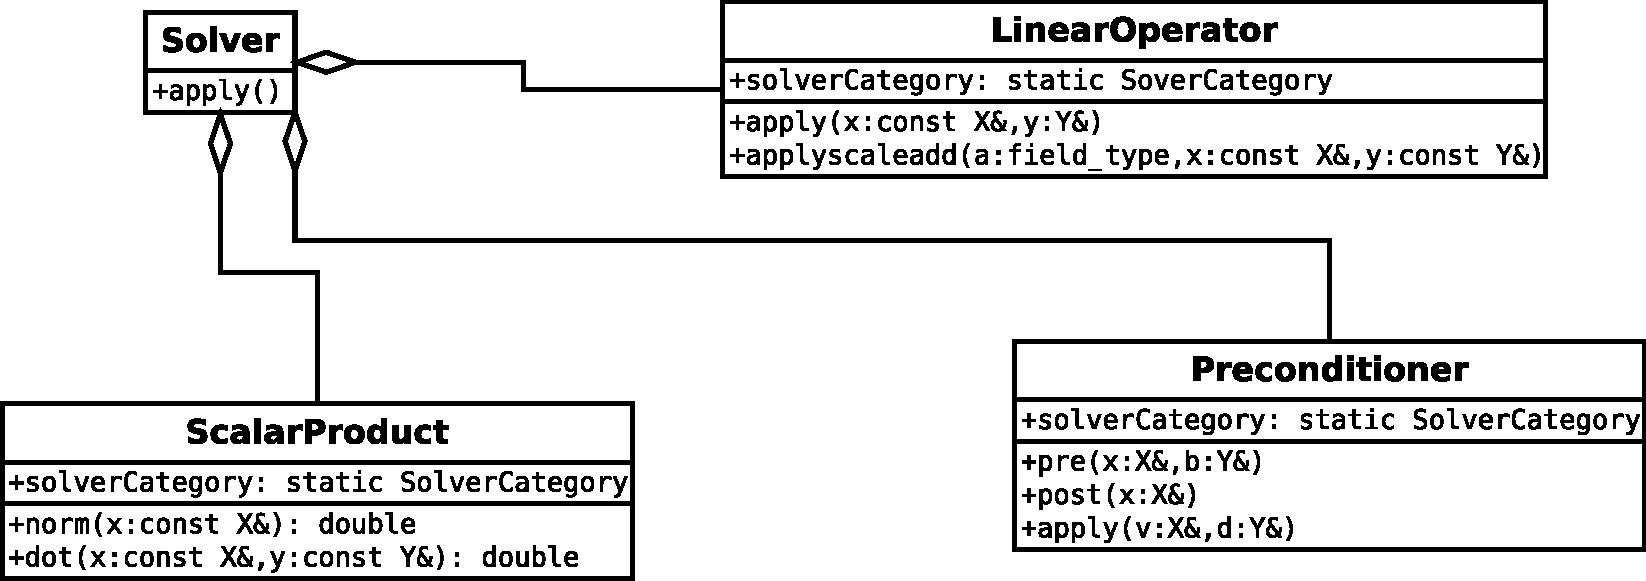
\includegraphics[width=\textwidth]{istlsolver}
\end{frame}

\begin{frame}
  \frametitle<presentation>{Parallel Solver Backends}

\begin{itemize}
\item ISTL solvers need to be provided a \lstinline!Preconditioner! (like Jacobi, SSOR or ILU), a
\lstinline!LinearOperator! (providing a matrix-vector product) and
a \lstinline!ScalarProduct!. The versions of these components have to fit together.
\item Parallel solver backends make sure that the correct implementations of
\lstinline!Preconditioner!, \lstinline!LinearOperator! and \lstinline!ScalarProduct!
are chosen matching the type of domain decomposition.
\item Different solver backends are provided for overlapping and nonoverlapping domain
decomposition.
\item The parallel solver backends can be found in the headers\newline \lstinline!dune/pdelab/backend/istl/ovlpistlsolverbackend.hh! and \newline
\lstinline!dune/pdelab/backend/istl/novlpistlsolverbackend.hh!,\newline 
which are automatically included by \lstinline!istl.hh!.
\end{itemize}

\end{frame}

%-----------------------------------------------------------------------------

\begin{frame}
\frametitle{Parallel Preconditioners}
\begin{itemize}
\item To run in parallel Conjugate Gradients (CG) and BiCGStab solvers have to be able to compute parallel matrix vector
products and scalar products.
\item As parallel preconditioners to the CG and BiCGStab solvers additive Schwarz methods can be used:
\begin{itemize}
\item In this schemes a local subproblem on each process is solved
where the values of the last iteration are used as Dirichlet constraints at the process boundary.
\item Different solvers can be choosen for the local problems\\ (e.g. a direct solver like SuperLU or some steps of an
iterative solver like SSOR).
\item In an overlapping decomposition the corrections are computed for the overlap at more than one process. The sum of the corrections multiplied with a relaxation
coefficient is applied.
\item With an overlapping Schwarz method the convergence is better the larger the overlap.
\end{itemize}
\item There exists also an algebraic multigrid preconditioner for overlapping as well as non-overlapping domain decomposition.
\end{itemize}
\end{frame}


\begin{frame}
  \frametitle{Parallel Solver Backends for Overlapping DD}
The linear solvers in this table are preconditioned with an overlapping domain decomposition
using the respective smoother or with a parallel algebraic multigrid scheme with an SSOR smoother (AMG).\medskip

\resizebox{0.9\textwidth}{!}{
\begin{tabular}{|l|l|l|}\hline
solver backend & smoother & linear solver\\\hline
\lstinline!ISTLBackend_OVLP_CG_SSORk<GFS,CC>! & SSOR & CG\\\hline
\lstinline!ISTLBackend_OVLP_CG_SuperLU<GFS,CC>! & SuperLU & CG\\\hline
\lstinline!ISTLBackend_OVLP_CG_UMFPack<GFS,CC>! & UMFPack & CG\\\hline
\lstinline!ISTLBackend_CG_AMG_SSOR<GO>! & AMG & CG\\\hline
\lstinline!ISTLBackend_OVLP_BCGS_SSORk<GFS,CC>! & SSOR & BiCGStab\\\hline
\lstinline!ISTLBackend_OVLP_BCGS_ILU0<GFS,CC>! & ILU0 & BiCGStab\\\hline
\lstinline!ISTLBackend_OVLP_BCGS_SuperLU<GFS,CC>! & SuperLU & BiCGStab\\\hline
\lstinline!ISTLBackend_BCGS_AMG_SSOR<GO>! & AMG & BiCGStab\\\hline
\end{tabular}}\medskip

\lstinline!ISTLBackend_OVLP_ExplicitDiagonal<GFS>! is a solver for explicit
time-steppers with (block-) diagonal mass matrix.

The template parameter \lstinline!GFS! is the grid function space, \lstinline!GO! is the grid operator, \lstinline!CC! is the type of the
constraints container (usually \lstinline!OverlappingConformingDirichletConstraints!).
\end{frame}

\begin{frame}[fragile]
  \frametitle{Overlapping Example}
\only<presentation>{\lstset{basicstyle=\scriptsize\ttfamily}}
  \begin{lstlisting}[breaklines=true,escapechar=!]
// 1. Create an overlapping grid
Dune::FieldVector<double,2> L(1.0);
Dune::FieldVector<int,2> N(16);
Dune::FieldVector<bool,2> periodic(false);
!\color{red}int overlap=2;!
Dune::YaspGrid<2> grid(L,N,periodic!\color{red},overlap!);
typedef Dune::YaspGrid<2>::LeafGridView GV;
const GV& gv=grid.leafView();

// 2. Create correctly constrained grid function space
typedef Dune::PDELab::Q1LocalFiniteElementMap<Coord,Real,dim> FEM;
FEM fem;
!\color{red}typedef Dune::PDELab::OverlappingConformingDirichletConstraints CON;!
typedef Dune::PDELab::ISTLVectorBackend<> VBE;
typedef Dune::PDELab::GridFunctionSpace<GV,FEM,CON,VBE> GFS;
GFS gfs(gv,fem);
\end{lstlisting}
\end{frame}
\begin{frame}[fragile]
\frametitle<presentation>{Overlapping Example Continued}
\only<presentation>{\lstset{basicstyle=\scriptsize\ttfamily}}
  \begin{lstlisting}[breaklines=true]
//  define problem parameters
typedef ConvectionDiffusionProblem<GV,Real> Param;
Param param;
typedef Dune::PDELab::BCTypeParam_CD<Param> B;
B b(gv,param);
typedef Dune::PDELab::DirichletBoundaryCondition_CD<Param> G;
G g(gv,param);

//  Compute constrained space
typedef typename GFS::template ConstraintsContainer<Real>::Type C;
C cg;
Dune::PDELab::constraints(b,gfs,cg);
// Make grid operator
typedef Dune::PDELab::ConvectionDiffusion<Param> LOP;
LOP lop(param,2);
typedef Dune::PDELab::ISTLMatrixBackend MBE;
typedef Dune::PDELab::GridOperator<GFS,GFS,LOP,MBE,double,double,double,C,C> GO;
GO go(gfs,cg,gfs,cg,lop);
\end{lstlisting}
\end{frame}
\begin{frame}[fragile]
\frametitle<presentation>{Overlapping Example Continued}
\only<presentation>{\lstset{basicstyle=\scriptsize\ttfamily}}
  \begin{lstlisting}[breaklines=true,escapechar=!]
//  Compute affine shift
typedef typename GO::Traits::Domain V;
V x(gfs,0.0);
Dune::PDELab::interpolate(g,gfs,x);
Dune::PDELab::set_nonconstrained_dofs(cg,0.0,x);

// 3. Choose a linear solver
!\color{red}typedef Dune::PDELab::ISTLBackend\_OVLP\_BCGS\_SuperLU<GFS,C> LS;!
LS ls(gfs,cg,5000,2);
...
\end{lstlisting}
\end{frame}

\begin{frame}
  \frametitle{Parallel Solver Backends for Nonoverlapping DD}
The linear solvers in this table are preconditioned with a nonoverlapping domain decomposition
using the respective smoother.\medskip

\resizebox{0.9\textwidth}{!}{
\begin{tabular}{|l|l|l|}\hline
solver backend & smoother & linear solver\\\hline
\lstinline!ISTLBackend_NOVLP_CG_NOPREC<GFS>! & -- & CG\\\hline
\lstinline!ISTLBackend_NOVLP_CG_Jacobi<GFS>! & Jacobi & CG\\\hline
\lstinline!ISTLBackend_NOVLP_CG_SSORk<GO>! & SSOR & CG\\\hline
\lstinline!ISTLBackend_NOVLP_CG_AMG_SSOR<GO>! & AMG & CG\\\hline
\lstinline!ISTLBackend_NOVLP_BCGS_NOPREC<GFS>! & -- & BiCGStab\\\hline
\lstinline!ISTLBackend_NOVLP_BCGS_Jacobi<GFS>! & Jacobi & BiCGStab\\\hline
\lstinline!ISTLBackend_NOVLP_BCGS_SSORk<GO>! & SSOR & BiCGStab\\\hline
\lstinline!ISTLBackend_NOVLP_BCGS_AMG_SSOR<GO>! & AMG & BiCGStab\\\hline
\end{tabular}}\medskip

\lstinline!ISTLBackend_NOVLP_ExplicitDiagonal! is a solver for explicit
time-steppers with (block-) diagonal mass matrix.

The template parameter is either \lstinline!GFS! the grid function space or \lstinline!GO! the grid operator depending on the preconditioner.
\end{frame}

\begin{frame}[fragile]
  \frametitle{Nonoverlapping example}
\only<presentation>{\lstset{basicstyle=\scriptsize\ttfamily}}
  \begin{lstlisting}[breaklines=true,escapechar=!]
// 1. Create an non-overlapping grid
Dune::FieldVector<double,2> L(1.0);
Dune::FieldVector<int,2> N(16);
Dune::FieldVector<bool,2> periodic(false);
!\color{red}int overlap=0; // overlap 0 as overlap elements are not assembled!
Dune::YaspGrid<2> grid(L,N,periodic!\color{red},overlap!);
typedef Dune::YaspGrid<2>::LeafGridView GV;
const GV& gv=grid.leafView();

// 2. Create correctly constrained grid function space
typedef Dune::PDELab::Q1LocalFiniteElementMap<Coord,Real,dim> FEM;
FEM fem;
!\color{red}typedef Dune::PDELab::NonoverlappingConformingDirichletConstraints<GV> CON;!
!\color{red}CON con(gv)!;
typedef Dune::PDELab::ISTLVectorBackend<> VBE;
typedef Dune::PDELab::GridFunctionSpace<GV,FEM,CON,VBE> GFS;
GFS gfs(gv,fem!\color{red},con!);
!\color{red}con.compute\_ghosts(gfs); // con stores indices of ghost dofs!
typedef ConvectionDiffusionProblem<GV,Real> Param;
Param param;
\end{lstlisting}
\only<presentation>{\lstset{basicstyle=\normalsize\ttfamily}}
\end{frame}
\begin{frame}[fragile]
\frametitle<presentation>{Nonoverlapping Example Continued}
\only<presentation>{\lstset{basicstyle=\scriptsize\ttfamily}}
  \begin{lstlisting}[breaklines=true]
typedef Dune::PDELab::BCTypeParam_CD<Param> B;
B b(gv,param);
typedef Dune::PDELab::DirichletBoundaryCondition_CD<Param> G;
G g(gv,param);
// Compute constrained space
typedef typename GFS::template ConstraintsContainer<Real>::Type C;
C cg;
Dune::PDELab::constraints(b,gfs,cg);

// Make grid operator
typedef Dune::PDELab::ConvectionDiffusion<Param> LOP;
LOP lop(param,2);
typedef Dune::PDELab::ISTLMatrixBackend MBE;
typedef Dune::PDELab::GridOperator<GFS,GFS,LOP,MBE,double,double,double,C,C,true> GO;
GO gos(gfs,cg,gfs,cg,lop);
\end{lstlisting}
\only<presentation>{\lstset{basicstyle=\normalsize\ttfamily}}
\end{frame}
\begin{frame}[fragile]
\frametitle<presentation>{Nonoverlapping Example Continued}
\only<presentation>{\lstset{basicstyle=\scriptsize\ttfamily}}
  \begin{lstlisting}[breaklines=true,escapechar=!]
// Compute affine shift
typedef typename GO::Traits::Domain V;
V x(gfs,0.0);
Dune::PDELab::interpolate(g,gfs,x);
Dune::PDELab::set_nonconstrained_dofs(cg,0.0,x);

// 3. Choose a linear solver
!\color{red}typedef Dune::PDELab::ISTLBackend\_NOVLP\_BCGS\_SSORk<GO> LS;!
LS ls(go,5000,3,2);
...
\end{lstlisting}

\end{frame}

\end{document}

